\documentclass{article}
\usepackage[utf8]{inputenc}
\usepackage[T1]{fontenc}
\usepackage{graphicx}
\usepackage{listings}
\usepackage{amsmath}
\usepackage{xcolor}
\usepackage{algorithmic}
\usepackage{amssymb}
\usepackage{float}
\usepackage{lipsum}
\usepackage{array}
\usepackage{enumitem}
\usepackage[margin=0.5in]{geometry}
\usepackage{titlesec}
\usepackage{geometry}
\usepackage{placeins}

\geometry{a4paper, margin=1in}

\begin{document}

    \setcounter{page}{2} 
    \tableofcontents
    \newpage

    \listoffigures

    \listoftables
    \newpage

    \section{Remerciements}
        Nous tenons à exprimer notre profonde gratitude à Mme LETRACHE et à M. KISSI pour les connaissances qu'ils nous ont transmises dans les modules de Technologie Web et de Modélisation UML. Nous leur sommes également reconnaissants pour leur soutien précieux, qui nous a permis de mettre en pratique ces acquis et de réussir notre projet. Grâce à leur aide, nous avons pu acquérir une expérience concrète dans la réalisation d'un projet.
    
    \newpage
    
    \section{Résumé}
        L'objectif de ce projet est de développer une application web en utilisant le langage PHP
        ,qui facilite les échanges,le partage d'informations et le support technique entre les collaborateurs d'une entreprise.
        Cette plateforme de collaboration permettra aux employés de poser des questions, 
        publier des annonces, partager des connaissances, gérer des formations et leurs profils.

        Le rapport commence par une introduction contextuelle, détaillant les spécifications fonctionnelles et techniques de l'application. Il décrit ensuite les différentes phases de conception et de réalisation. Les outils et technologies employés sont également présentés, avec un chapitre spécifiquement consacré à la mise en œuvre concrète de l'application.
    
    \section{Contexte du projet}
        \subsection{Introduction}
            Tout projet de développement logiciel réussi repose sur la collaboration entre les développeurs au sein d'une entreprise. Cela leur offre la possibilité de transmettre leurs connaissances, de repérer aisément les erreurs et de trouver des solutions plus novatrices. Les développeurs peuvent optimiser la répartition des différentes tâches et garantir une intégration adéquate de chaque partie du code avec le reste du projet. Cependant, afin que cette collaboration soit réellement fluide, il est nécessaire d'avoir quelque chose en place qui facilite naturellement la communication et la coordination. C'est à ce moment-là qu'une application web intervient. Ce genre d'outil regroupe les échanges, le suivi des tâches, le partage de fichiers et la gestion des versions de code en un seul endroit, de manière à ce que tous les utilisateurs puissent y accéder.
        
        \subsection{Objectifs du projet}
            L'objectif principal de ce projet est de développer une application web de collaboration pour les entreprises, en utilisant le langage PHP. Les objectifs spécifiques incluent :

            \begin{itemize}
                \item \textbf{Faciliter la communication} : Permettre aux collaborateurs de poser des questions et d'obtenir des réponses rapidement.
                \item \textbf{Partager des informations} : Offrir une plateforme pour publier des annonces et partager des connaissances.
                \item \textbf{Support technique} : Proposer un support technique intégré pour aider les employés avec leurs problèmes informatiques.
                \item \textbf{Gestion des formations} : Permettre la gestion et le suivi des formations internes.
                \item \textbf{Gestion des profils} : Offrir la possibilité de créer et de gérer les profils des employés.
            \end{itemize}

        \subsection{Distribution des tâches}
            Aucune tâche n'a été réalisée par un seul membre du groupe. Le travail est dédié à tous les membres du groupe, 
            et chaque tâche est vérifiée par tous les membres du groupe.
            Cette distribution concerne la réalisation initiale de la tâche (premier commit), puis on améliore cette dernière si nécessaire.\newline
            si on ne spécifie pas la partie(backend ou frontend), donc le membre du groupe travaille sur les deux parties.\newline
            \begin{table}[h!]
                \centering
                \begin{tabular}{|l|l|}
                    \hline
                    Partie &
                    Tâche \\
                    \hline
                    Conception  &
                    Diagramme de classe (CHROQUI) \\
                                &
                    MCD (CHROQUI) \\
                                &
                    Diagrammes des cas d'utilisations (AMKASSOU) \\
                                &
                    Diagrammes d'états transitions (CHROQUI) \\
                                &
                    Diagramme de Sequence (HERAK) \\
                                &
                    Diagramme d'activité (HERAK) \\
                    \hline
                    réalisation &
                    BDD, Les profile (frontend), systéme de notification, systéme des états des questions,\\
                                &
                    Modération des questions (AMKASSOU). \\
                                &
                    Pages d'accueil, Login et logout et inscription, questions, incription\\
                                &
                    dans les formations et annonces, like et dislike,\\
                                &
                    gestion profile Admin(backend),la recherche et systéme des états des formation (CHROQUI). \\
                                &
                    Pages des projets, evenements, base de connaissances, formations,\\
                                &
                    dashboard de l'Admin, gestion profile collaborateurs(backend) et la recherche (HERAK). \\
                    \hline
                \end{tabular}
                \caption{Distribution des tâches}
            \end{table}
            \FloatBarrier
        \subsection{Conclusion}
            En conclusion, ce projet vise à créer une application web en PHP qui répond aux besoins de communication et de collaboration au sein des entreprises. En facilitant les échanges d'informations, le partage de connaissances et le support technique, cette plateforme contribuera à améliorer la productivité et l'efficacité des équipes. La gestion des formations et des profils des employés permettra également une meilleure organisation et un suivi plus rigoureux des compétences. Grâce à une mise en œuvre soignée et à l'utilisation des technologies appropriées et enrichissement des fonctionnalités, cette application promet de devenir un outil indispensable pour toute entreprise cherchant à optimiser ses processus internes.
    
    \section{Conception}
        \subsection{Introduction}
            Dans cette partie on va présentés la conception du projet, réalisée a l'aide des Diagrammes UML.
            section*{Analyse des Besoins Fonctionnels et Non-Fonctionnels}

        \subsection{Spécifications Fonctionnelles du Projet}
            \begin{enumerate}
                \item \textbf{Forum Question/Réponse :}
                \begin{itemize}
                    \item Offrir un espace de partage et de support aux collaborateurs.
                \item Fonctionnalités requises :
                    \begin{itemize}
                        \item Publication d'une question avec titre, description et projet concerné (optionnel).
                        \item Passage d'état : Nouveau → En cours → Complété → résolu ou Relancé.
                        \item Notification pour l'émetteur lorsque complété.
                        \item Réactions aux réponses avec Like/Dislike, commentaires et notes.
                    \end{itemize}
                \end{itemize}
                
                \item \textbf{Gestion des Annonces :}
                \begin{itemize}
                    \item Publication d'annonces pour formations, meetings, événements.
                    \item Informations requises : titre, description, date, lien, image, projet concerné (optionnel).
                \end{itemize}
                
                \item \textbf{Base de Connaissances :}
                \begin{itemize}
                    \item Partage de connaissances techniques.
                    \item Informations requises : titre, description, catégorie (prédéfinies), mots clés (3).
                \end{itemize}
                
                \item \textbf{Gestion des Formations :}
                \begin{itemize}
                    \item Planification et organisation de formations en ligne.
                    \item Informations requises : thème, description, formateur, dates, lien.
                    \item Inscription des collaborateurs intéressés avec notification au créateur.
                \end{itemize}
                
                \item \textbf{Gestion des Profils :}
                \begin{itemize}
                    \item Chaque collaborateur a un compte avec gestion de profil.
                    \item Informations personnelles, compétences et leurs niveau de maîtrise, rôles dans les projets.
                \end{itemize}
                
                \item \textbf{Gestion des Projets et Compétences :}
                \begin{itemize}
                    \item Gérée par l'administrateur.
                    \item Définition et mise à jour des projets, rôles, compétences et niveaux de maîtrise.
                \end{itemize}
            \end{enumerate}
            
        \subsection{Spécifications Non-Fonctionnelles du Projet}
            \begin{itemize}
                \item \textbf{Sécurité :} Authentification sécurisée pour l'accès aux fonctionnalités.
                \item \textbf{Performance :} Réponses rapides aux requêtes des utilisateurs.
                \item \textbf{Extensibilité :} Capacité à ajouter de nouvelles fonctionnalités et modules.
                \item \textbf{Maintenance :} Facilité de maintenance et de mise à jour de l'application.
                \item \textbf{Accessibilité :} Interface utilisateur intuitive et compatible avec différents navigateurs.
                \item \textbf{Scalabilité :} Gestion efficace d'un nombre croissant d'utilisateurs et de données.
            \end{itemize}

        \subsection{Les acteurs du systéme}  
            \begin{itemize}
                \item \textbf{administrateur} : L'utilisateur qui a le droit d'ajouts et suppressions de projets,compétences et niveaux de maîtrise,la gestion des utilisateurs,supervision des formations,questions et annonces, et de la consulation du dashboard .
                \item \textbf{collaborateurs} : L'utilisateur qui a le droit de publier des question,réponses,des annonces,des base de connaissances,des formations, de définir ses niveaux de maîtrise,ses rôles dans les projets.
            \end{itemize}

        \subsection{les Diagrammes UML}
            Tous les acteurs et leurs tâches sont présentés dans les diagrammes suivants :
            
            \subsubsection{Diagrammes de Classe}
                \begin{figure}[h!]
                    \centering
                    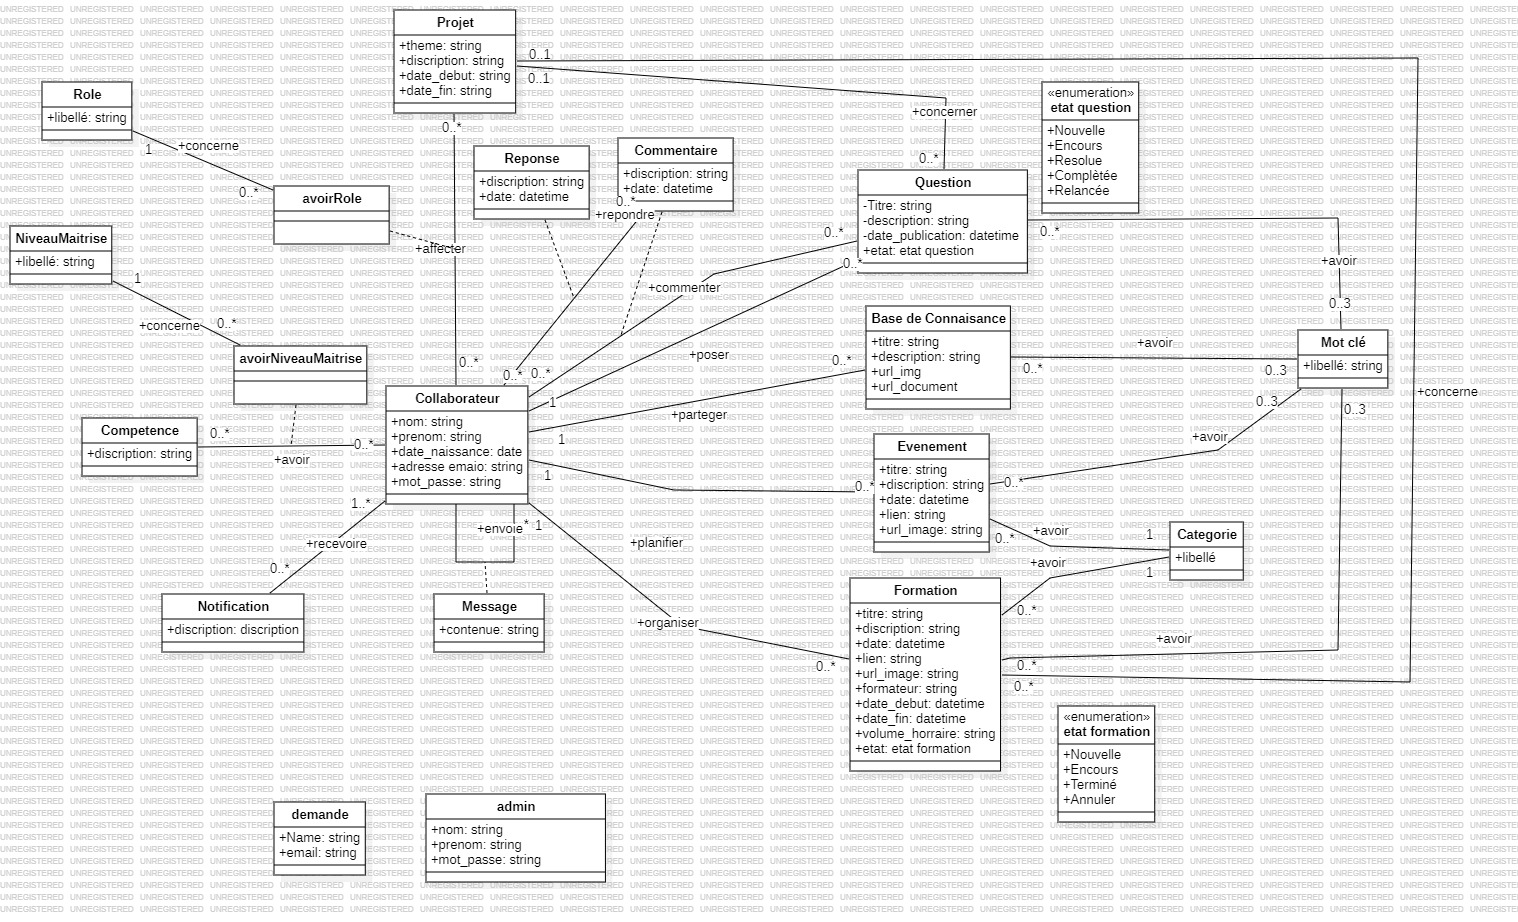
\includegraphics[width=1.0\textwidth]{assets/diagrammes/class.jpg}
                    \caption{Diagramme de Classe}
                \end{figure}
                \FloatBarrier   
            \subsubsection{MCD}
                % \begin{center}
                %     \centering
                %     \includegraphics[width=0.8\textwidth]{diagrammes/}
                % \end{center}

            \subsubsection{Diagrammes des cas d'utilisations}
                \textbf{Diagramme des cas d'utilisations} : Tous les cas d'utilisation sont associés avec l'association d'inclusion « include » au 
                cas d'utilisation « S'authentifier » :
                
                Pour les questions: 
                \begin{figure}[h!]
                    \centering
                    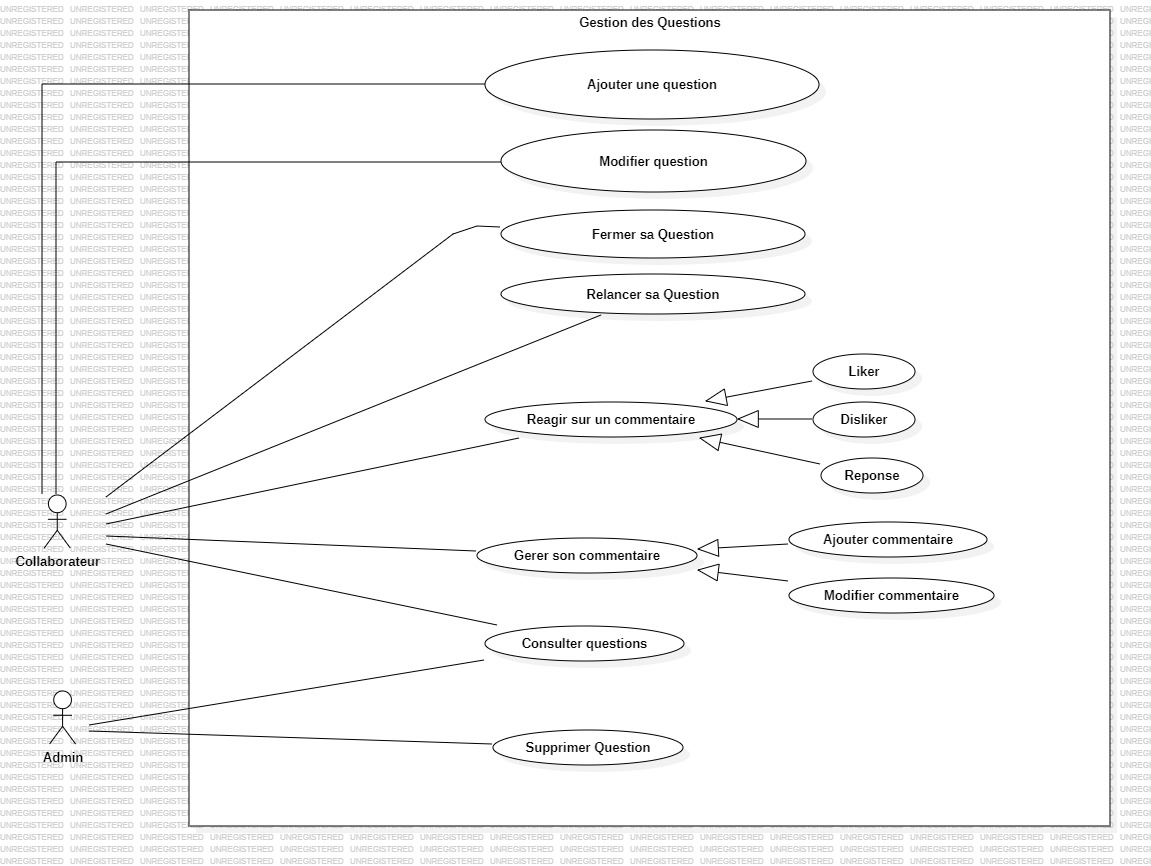
\includegraphics[width=0.8\textwidth]{assets/diagrammes/jpg/Model1!useCaseQuestion_0.jpg}
                    \caption{Diagramme des cas d'utilisations - Question}
                \end{figure}
                
                \FloatBarrier
                
                Les evenements : 
                \begin{figure}[h!]
                    \centering
                    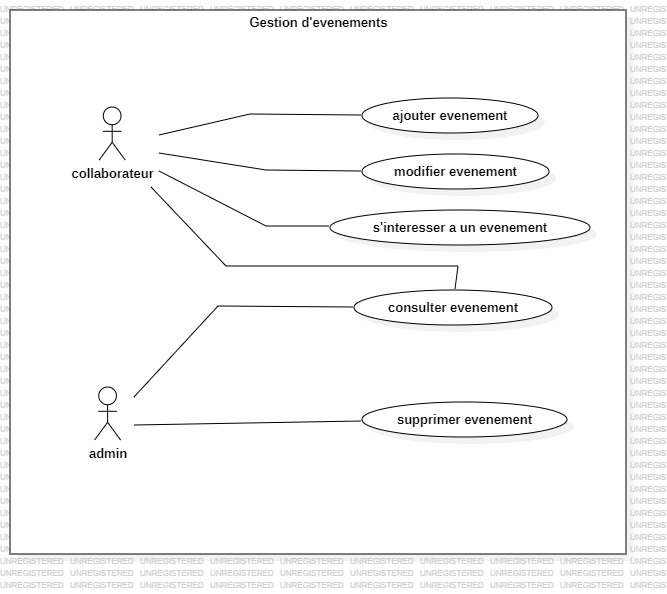
\includegraphics[width=0.8\textwidth]{assets/diagrammes/jpg/Model2!UseCaseEvent_1.jpg}
                    \caption{Diagramme des cas d'utilisations - Event}
                \end{figure}
                
                \FloatBarrier
                
                La base des connaissances
                \begin{figure}[h!]
                    \centering
                    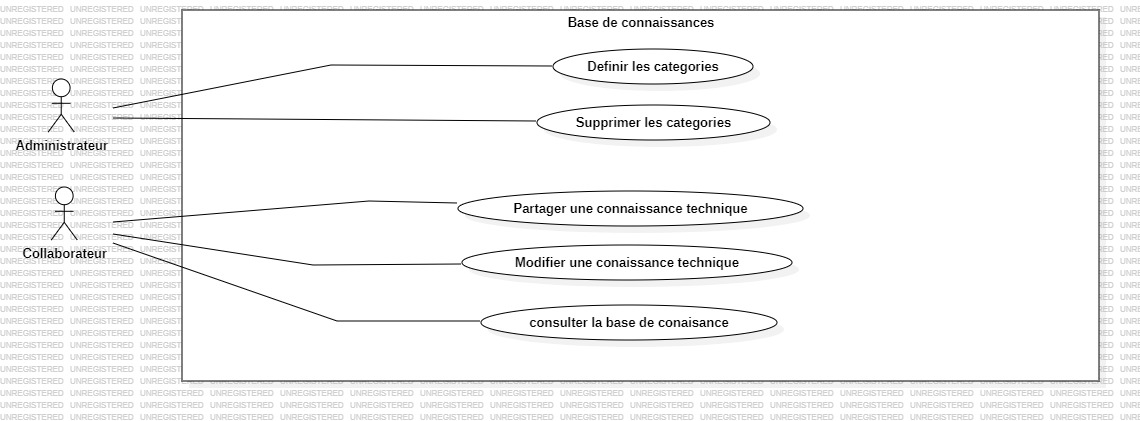
\includegraphics[width=0.8\textwidth]{assets/diagrammes/jpg/Model3!UseCaseDoc_2.jpg}
                    \caption{Diagramme des cas d'utilisations - base de connaissances}
                \end{figure}
                
                \FloatBarrier
                
                Les formations
                \begin{figure}[h!]
                    \centering
                    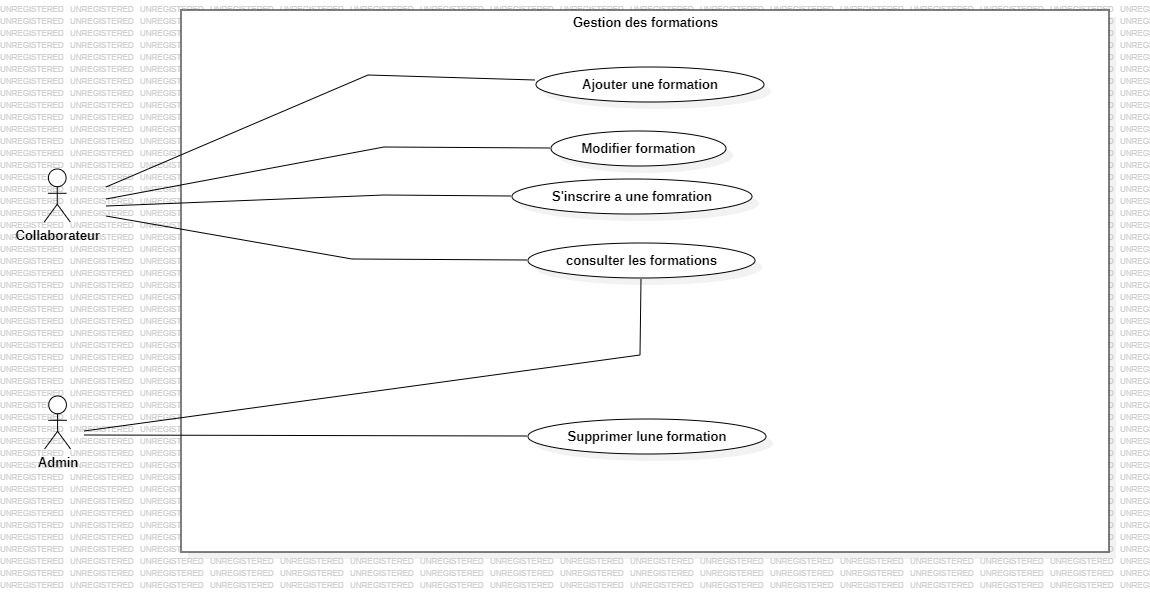
\includegraphics[width=0.8\textwidth]{assets/diagrammes/jpg/Model4!UseCaseFormation_3.jpg}
                    \caption{Diagramme des cas d'utilisations - Formation}
                \end{figure}
                
                \FloatBarrier
                
                Profile collaborateur :
                \begin{figure}[h!]
                    \centering
                    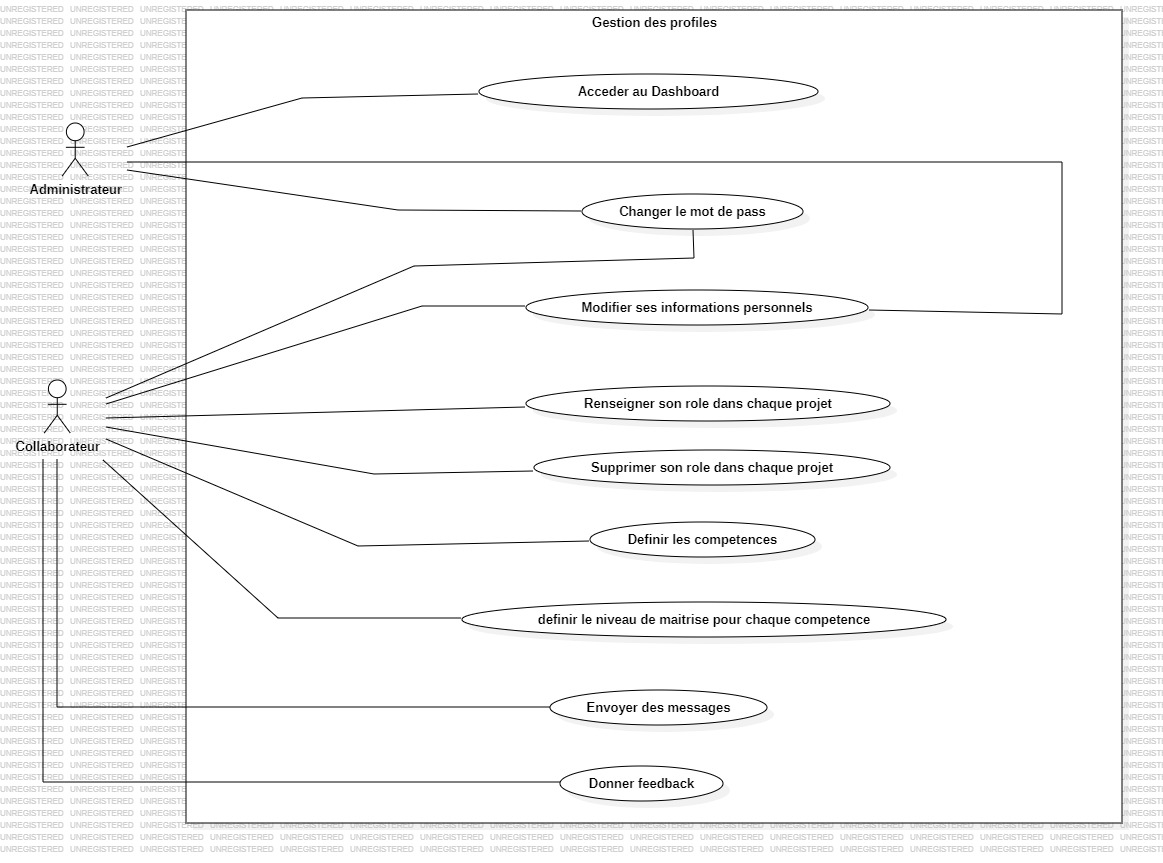
\includegraphics[width=0.8\textwidth]{assets/diagrammes/jpg/Model5!UseCaseCollab_4.jpg}
                    \caption{Diagramme des cas d'utilisations - Collaboration}
                \end{figure}
                
                \FloatBarrier
                
                Les projets :
                \begin{figure}[h!]
                    \centering
                    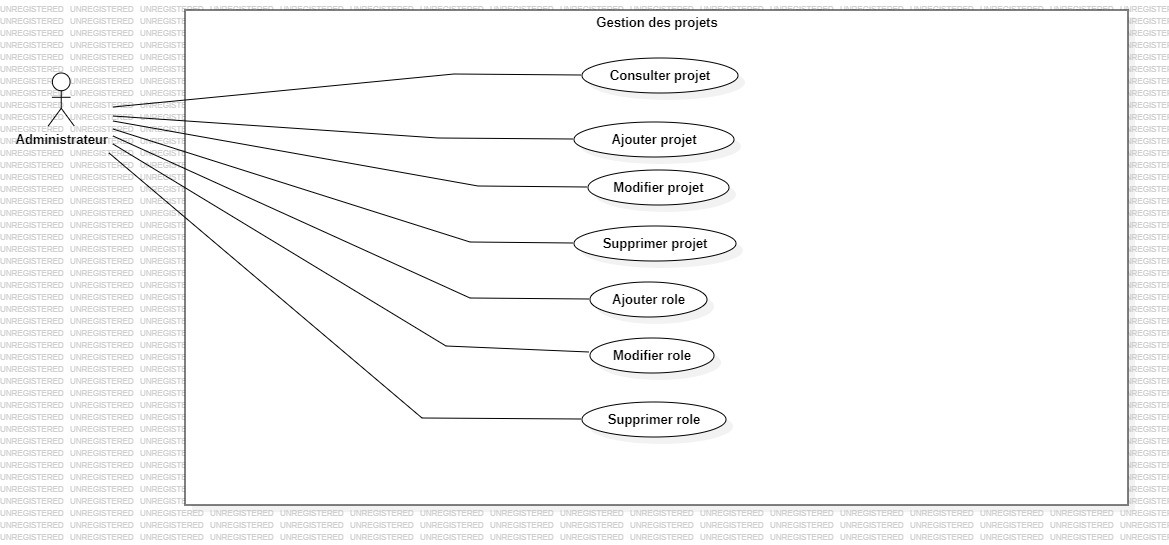
\includegraphics[width=0.8\textwidth]{assets/diagrammes/jpg/Model6!UseCaseProject_5.jpg}
                    \caption{Diagramme des cas d'utilisations - Projet}
                \end{figure}
                \FloatBarrier
            
            \subsubsection{Diagrammes d'Etats Transitions}
                Pour les états d'une question :
                \begin{figure}[h!]
                    \centering
                    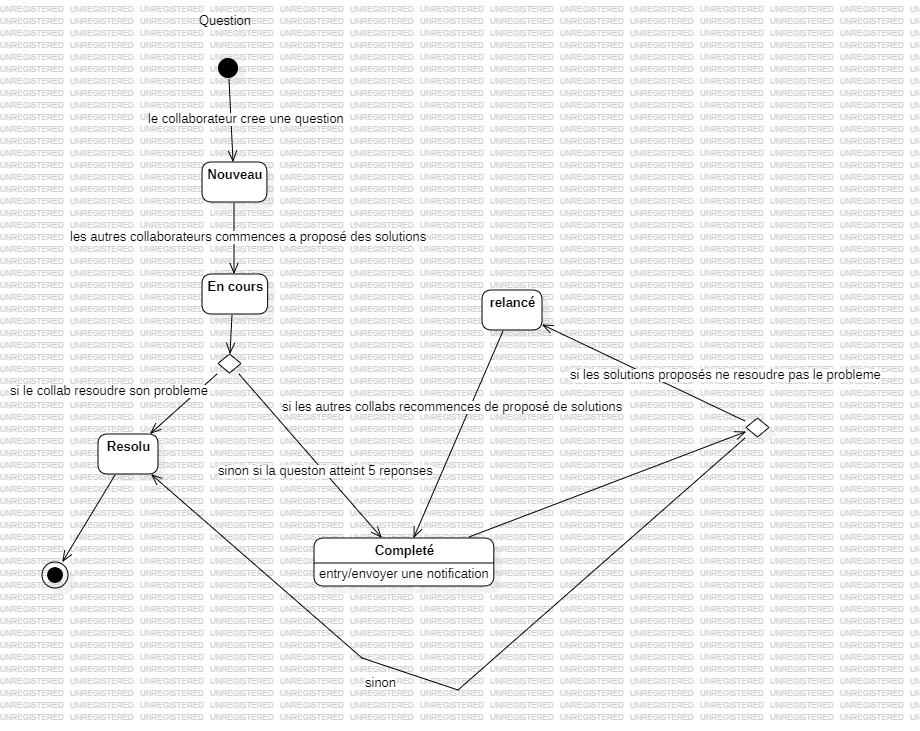
\includegraphics[width=0.8\textwidth]{assets/diagrammes/jpg/StateMachine1!Question_0.jpg}
                    \caption{Diagramme d'Etats Transitions - Question}
                \end{figure}
                \FloatBarrier
                Pour les états d'une formation :
                \begin{figure}[h!]
                    \centering
                    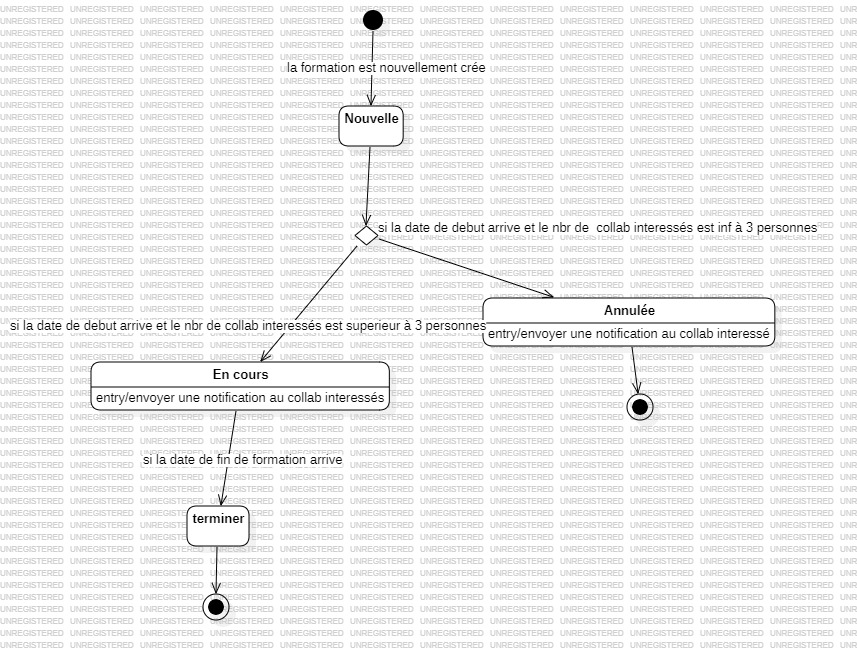
\includegraphics[width=0.8\textwidth]{assets/diagrammes/jpg/StateMachine2!Formation_1.jpg}
                    \caption{Diagramme d'Etats Transitions - Formation}
                \end{figure}
                \FloatBarrier
            
            \subsubsection{Diagramme de Sequence}
                % \begin{center}
                %     \includegraphics[width=0.8\textwidth]{diagrammes/}
                % \end{center}

            \subsubsection{Diagramme d'Activité}
                \begin{figure}[h!]
                    \centering
                    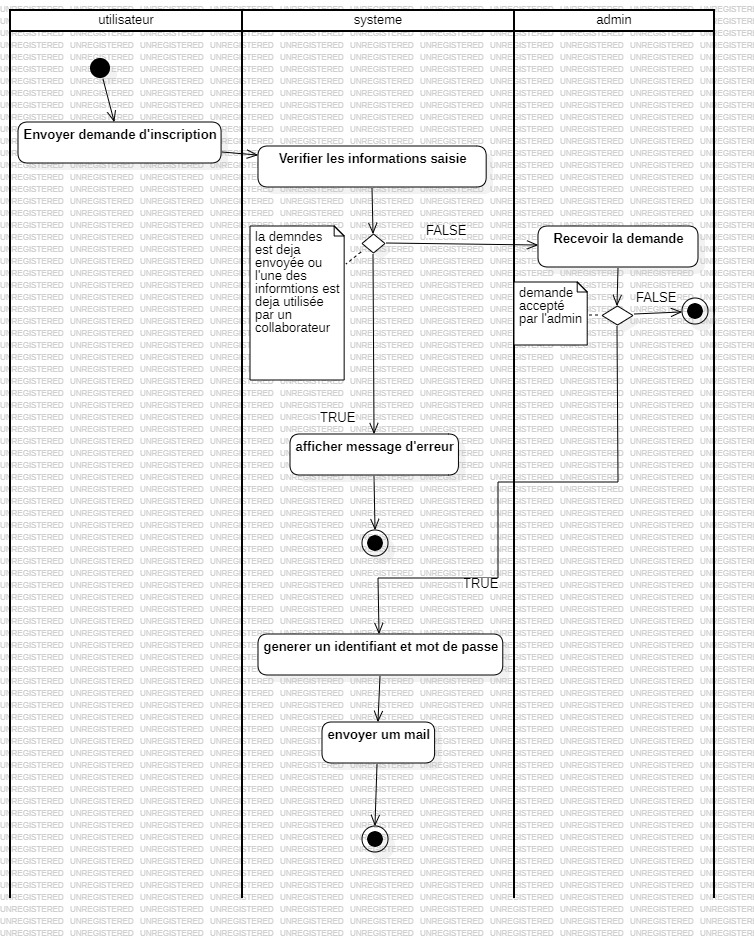
\includegraphics[width=0.8\textwidth]{assets/diagrammes/ActivityDiagram.jpg}
                    \caption{Diagramme d'activité - inscription}
                \end{figure}
                \FloatBarrier
        
        \subsection{Conclusion}
            la partie conception de ce projet est finie. On passe maintenant vers la réalisation, mais avant on doit savoir l'importance de la conception,
            la conception dans un projet informatique joue un rôle fondamental pour assurer le succès et la qualité du produit final, 
            en alignant les besoins et les objectifs avec une structure technique et fonctionnelle bien définie. 
            Elle constitue une étape préalable essentielle avant le développement proprement dit, 
            permettant de poser des bases solides pour la réalisation du projet.
            
    \section{réalisation}
        \subsection{Introduction}
            Dans cette partie on va présenter la réalisation du projet, avec les technologies,logiciel et bibliotheques utilisées.
        
        \subsection{Outils de développement}
            
            \subsubsection{Equipement logiciel}
                \begin{table}[h!]
                    \centering
                    \begin{tabular}{|m{2cm}|m{12cm}|}
                        \hline
                        
\includegraphics[width=2cm]{assets/logos/vscode.png} &
                        \textbf{Visual Studio Code} :
                        
                        Visual Studio Code (VS Code) est un éditeur de code source gratuit, léger et extrêmement populaire développé par Microsoft. Il offre un large éventail de fonctionnalités et de plugins qui en font un outil polyvalent pour les développeurs. \\
                        \hline
                        
\includegraphics[width=2cm]{assets/logos/wamp.jpg} &
                        \textbf{WAMP Server} :
                        
                        Pour que nous puissions fonctionner localement des scripts PHP, WAMP est l'abrégé de Windows, Apache, MySQL et PHP. On a choisi d'utiliser WampServer parce qu'il facilite le travail via une interface d'administration ainsi que gérer des bases des données. Il contient les dernières versions existantes des logiciels comme Apache et PHP. \\
                        \hline
                        
\includegraphics[width=2cm]{assets/logos/OIP.jpg} &
                        \textbf{PhpMyAdmin} :
                        
                        PHPMyAdmin : interface web en PHP pour administrer à distance les SGBD MySQL et MariaDB. Il permet d'administrer les bases de données, les tables et leurs champs, les index, les clés primaires et étrangères, les utilisateurs de la base et leurs permissions et importer ou exporter les données dans divers formats. \\
                        \hline
                        
\includegraphics[width=2cm]{assets/logos/mysql_PNG22.png} &
                        \textbf{MySQL} :
                        
                        MySQL est un serveur de bases de données relationnelles SQL développé dans un souci de performances élevées en lecture, ce qui signifie qu'il est davantage orienté vers le service de données déjà en place que vers celui de mises à jour fréquentes et fortement sécurisées. \\
                        \hline
                        
\includegraphics[width=2cm]{assets/logos/staruml-icon.png} &
                        \textbf{StarUML} :
                        
                        StarUML est un outil de génie logiciel dédié à la modélisation UML. Il est multiplateforme et fonctionne sous Windows, Linux et MacOS. \\
                        \hline
                        
\includegraphics[width=2cm]{assets/logos/github-mark.png} &
                        \textbf{GitHub} :
                        
                        GitHub est une plateforme en ligne populaire qui offre des fonctionnalités de gestion de versions et de collaboration pour les projets de développement de logiciels. \\
                        \hline
                    \end{tabular}
                    \caption{Equipement logicielles}
                \end{table}
            \FloatBarrier
            \subsubsection{Langages d'implémentation}
                \begin{table}[h!]
                    \centering
                    \begin{tabular}{|m{2cm}|m{12cm}|}
                        \hline
                        
\includegraphics[width=2cm]{assets/logos/PHP_logo.png} &
                        \textbf{PHP} :
                        
                        PHP : (HyperText Preprocessor) langage de programmation libre, principalement utilisé pour produire des pages web dynamiques via un serveur HTTP, mais pouvant également fonctionner comme n'importe quel langage interprété de façon locale. \\
                        \hline
                        
\includegraphics[width=2cm]{assets/logos/js.jpg} &
                        \textbf{JavaScript} :
                        
                        JavaScript : un langage de programmation qui permet de créer du contenu mis à jour de façon dynamique, de contrôler le contenu multimédia, d'animer des images, et tout ce à quoi on peut penser. Bon, peut-être pas tout, mais vous pouvez faire bien des choses avec quelques lignes de JavaScript. \\
                        \hline
                        
\includegraphics[width=2cm]{assets/logos/html.jpg} &
                        \textbf{HTML} :
                        
                        HTML : (HyperText Markup Language) langage de balisage permettant d'écrire de l'hypertexte. HTML permet également de structurer sémantiquement et de mettre en forme le contenu des pages, d'inclure des ressources multimédias dont des images, des formulaires, et des éléments programmables tels que des applets. Il permet de créer des documents interopérables avec des équipements très variés de manière conforme aux exigences de l'accessibilité du web. \\
                        \hline
                        
\includegraphics[width=2cm]{assets/logos/css.png} &
                        \textbf{CSS} :
                        
                        CSS est un langage de style dont la syntaxe est simple mais son effet est remarquable, il s'intéresse à la mise en forme du contenu intégré avec du HTML. \\
                        \hline
                    \end{tabular}
                    \caption{Langages d'implémentation}
                \end{table}
            \FloatBarrier
            \subsubsection{Frameworks et bibliothèques}
                \begin{table}[h!]
                    \centering
                    \begin{tabular}{|m{2cm}|m{12cm}|}
                        \hline
                        
\includegraphics[width=2cm]{assets/logos/OIP (1).jpg} &
                        \textbf{Bootstrap} :
                        
                        Bootstrap : Collection d'outils utiles à la création du design (graphisme, animation et interactions avec la page dans le navigateur, etc.) de sites et d'applications web. C'est un ensemble qui contient des codes HTML et CSS, des formulaires, boutons, outils de navigation et autres éléments interactifs, ainsi que des extensions JavaScript en option. \\
                        \hline
                        
\includegraphics[width=2cm]{assets/logos/jq.png} &
                        \textbf{JQuery} :
                        
                        JQuery : Bibliothèque JavaScript libre et multiplateforme créée pour faciliter l'écriture de scripts côté client dans le code HTML des pages web. \\
                        \hline
                        
\includegraphics[width=2cm]{assets/logos/ajax.png} &
                        \textbf{AJAX} :
                        
                        AJAX : architecture logicielle permettant de créer des pages et des applications web capables d'interagir avec l'utilisateur et/ou d'autres applications sans qu'il soit nécessaire de recharger cette page dans le navigateur web du poste client. AJAX s'appuie sur des technologies présentes dans les différents navigateurs web, dont JavaScript (JS) et XML. \\
                        \hline
                    \end{tabular}
                    \caption{Frameworks et bibliothèques}
                \end{table}
            \FloatBarrier
        \subsection{Conclusion}
            Durant ce projet, nous avons eu l'opportunité de travailler avec une gamme variée de technologies, notamment PHP, JavaScript, HTML, CSS, Bootstrap, JQuery, AJAX, GitHub, Visual Studio Code, PhpMyAdmin et WAMP Server. 

            Ces outils nous ont permis d'appliquer concrètement les connaissances acquises dans le cadre du module de Technologie Web. Nous considérons ces technologies comme les fondements du développement web et, grâce à ce projet, nous avons établi une base solide pour l'exploration de nouvelles technologies à l'avenir.
    
    \section{Mise en oeuvre}
        Dans cette section, nous allons détailler la mise en œuvre du projet. Cet espace de collaboration peut être divisé en deux parties : la première, dédiée aux collaborateurs, et la seconde, réservée à l'administration.
        \subsection{Page d'accueil}
                Une page partager entre les deux acteurs, vise a rediriger l'utilisateur vers la page de connexion, quoi qu'il soit un admin ou collaborateur.
                \begin{figure}[h!]
                    \centering
                    
\includegraphics[width=0.8\textwidth]{assets/webSite/homePage.png}
                    \caption{Page d'accueil}
                \end{figure}
                \FloatBarrier
        \subsection{Espace collaborateur}
            \subsubsection{Page de Connexion}
                La connexion est utilisée pour assurer la session, et rediriger l'utilisateur vers la page de profil, En PHP, les sessions sont utilisées pour stocker des informations sur l'utilisateur de manière persistante pendant qu'il navigue sur le site. Cela permet, par exemple, de maintenir un utilisateur connecté entre différentes pages. Chaque session est identifiée de manière unique par un identifiant de session (session ID) qui est généralement stocké dans un cookie côté client.
                Ainsi, elle assure que l'utilisateur ne se connecte qu'une seule fois sur le site, est que s'il n'a jamais de session, il ne peut pas acceder a la platforme.
                \begin{figure}[h!]
                    \centering
                    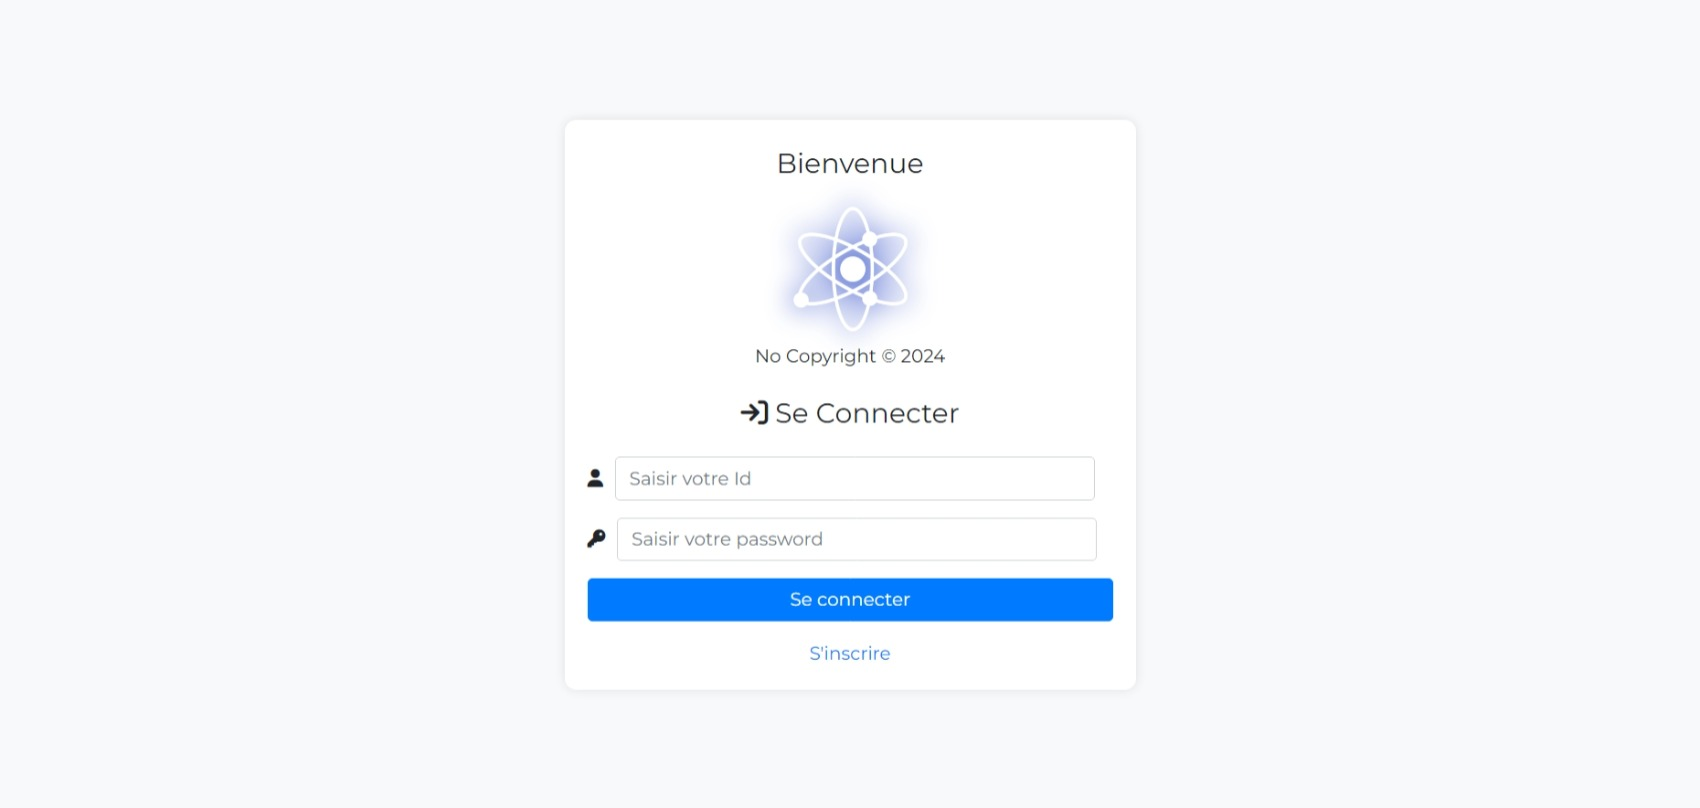
\includegraphics[width=0.7\textwidth]{assets/webSite/loginCollab.jpeg}
                    \caption{Page de Connexion}
                \end{figure}
                \FloatBarrier
            \subsubsection{Page d'Inscription}
                Cas ou le membre souhaite s'inscrire sur le site, on lui redirigera vers la page d'inscription, ou il envoie une demande avec ses informations personnel, et le membre sera inscrit sur le site si l'Admin accepte la demande.
                Chaque membre accepté recoie un email de confirmation, qui contient les informations de connexion.
                \begin{figure}[h!]
                    \centering
                    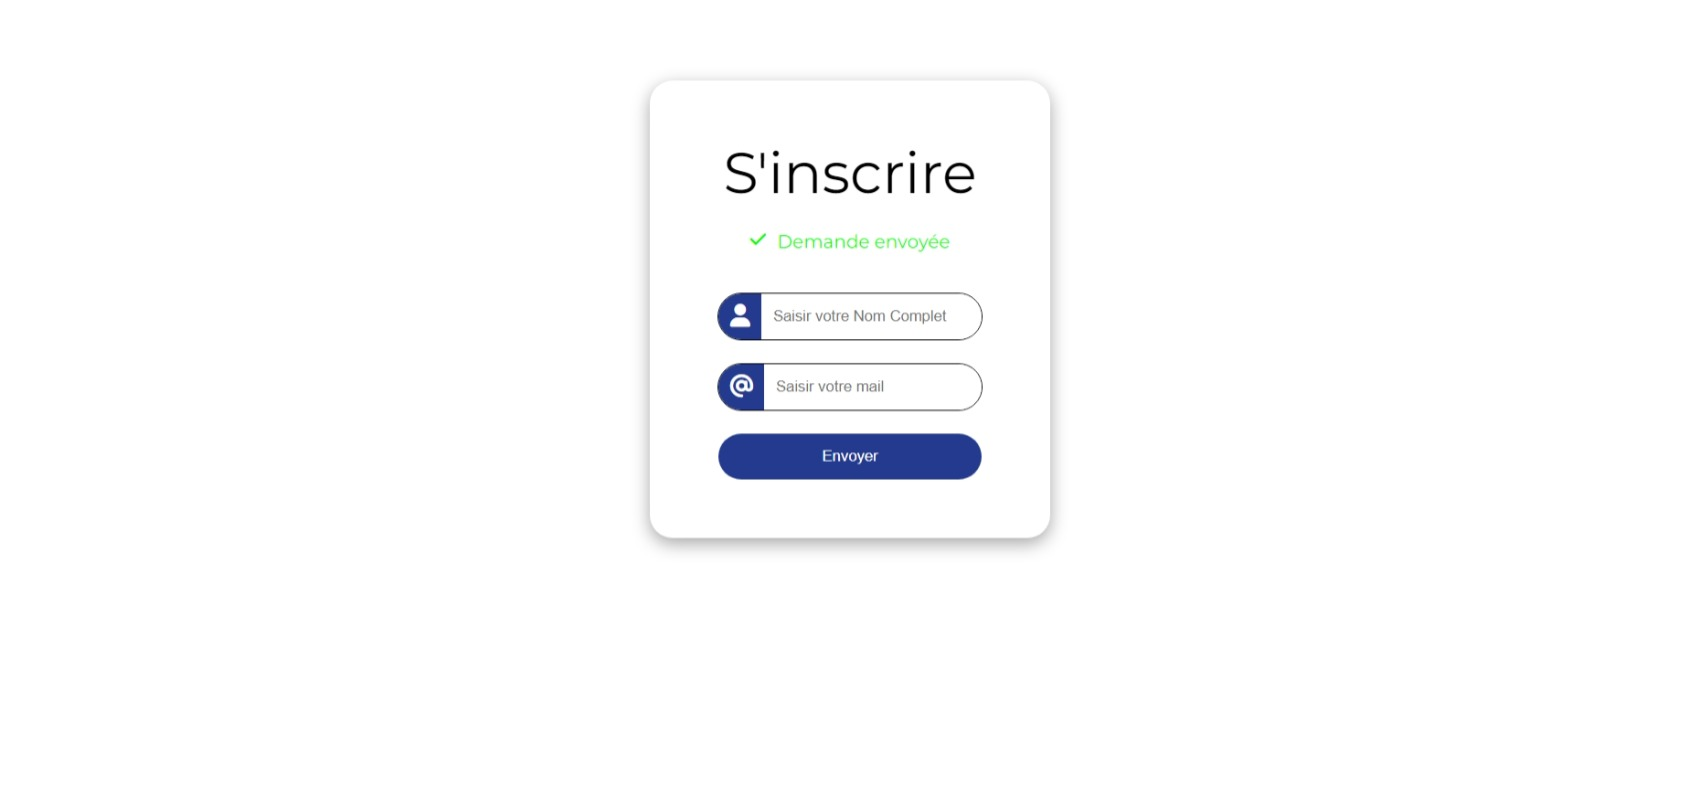
\includegraphics[width=0.3\textwidth]{assets/webSite/envoieDemande.jpeg}
                    \caption{Page d'Inscription}
                \end{figure}
                \FloatBarrier
            \subsubsection{Page de profil}
                Chaque collaborateur a une page de son profile, ou il peux voir les question qu'il a poser,les formations,evenements qu'il interresse, plus une gestion de ses questions.
                \begin{figure}[h!]
                    \centering
                    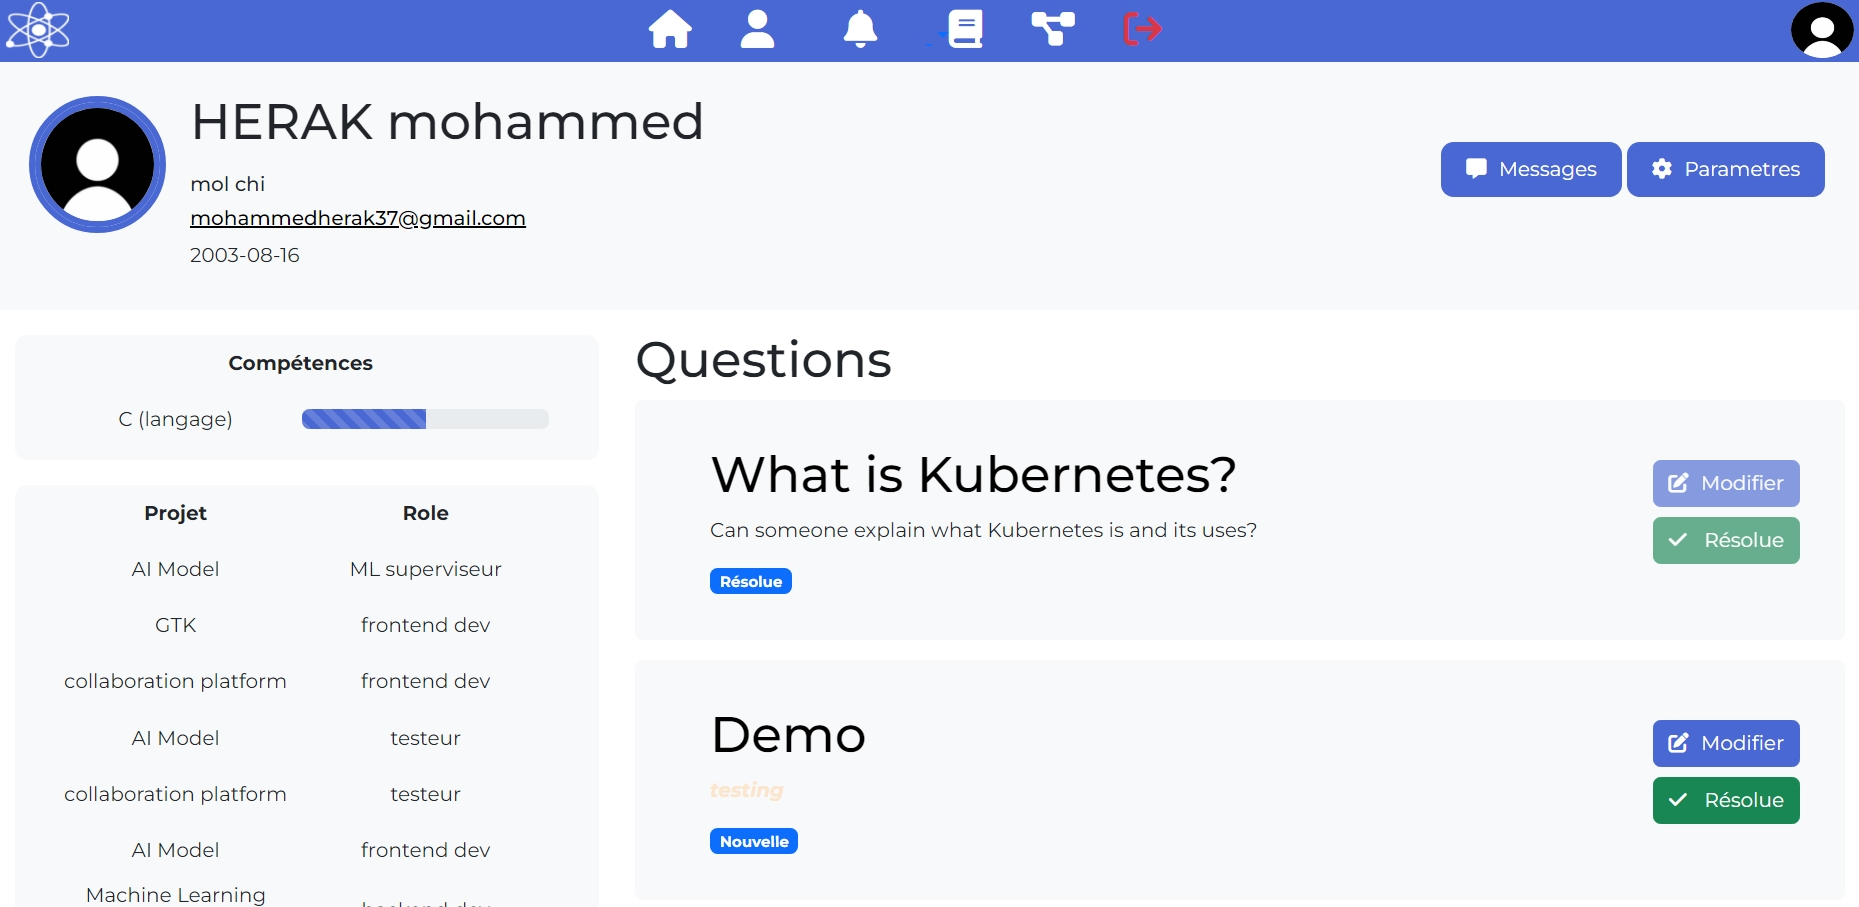
\includegraphics[width=0.8\textwidth]{assets/webSite/profielPage.jpeg}
                    \caption{Page de profil}
                \end{figure}
                \FloatBarrier
            \subsubsection{Page de modification du profil}
                Depuis le profile et en cliquant sur un simple bouton, le collaborateur se redirige vers une page ou il peut modifier la tottalite des informations de son profile.
                \begin{figure}[h!]
                    \centering
                    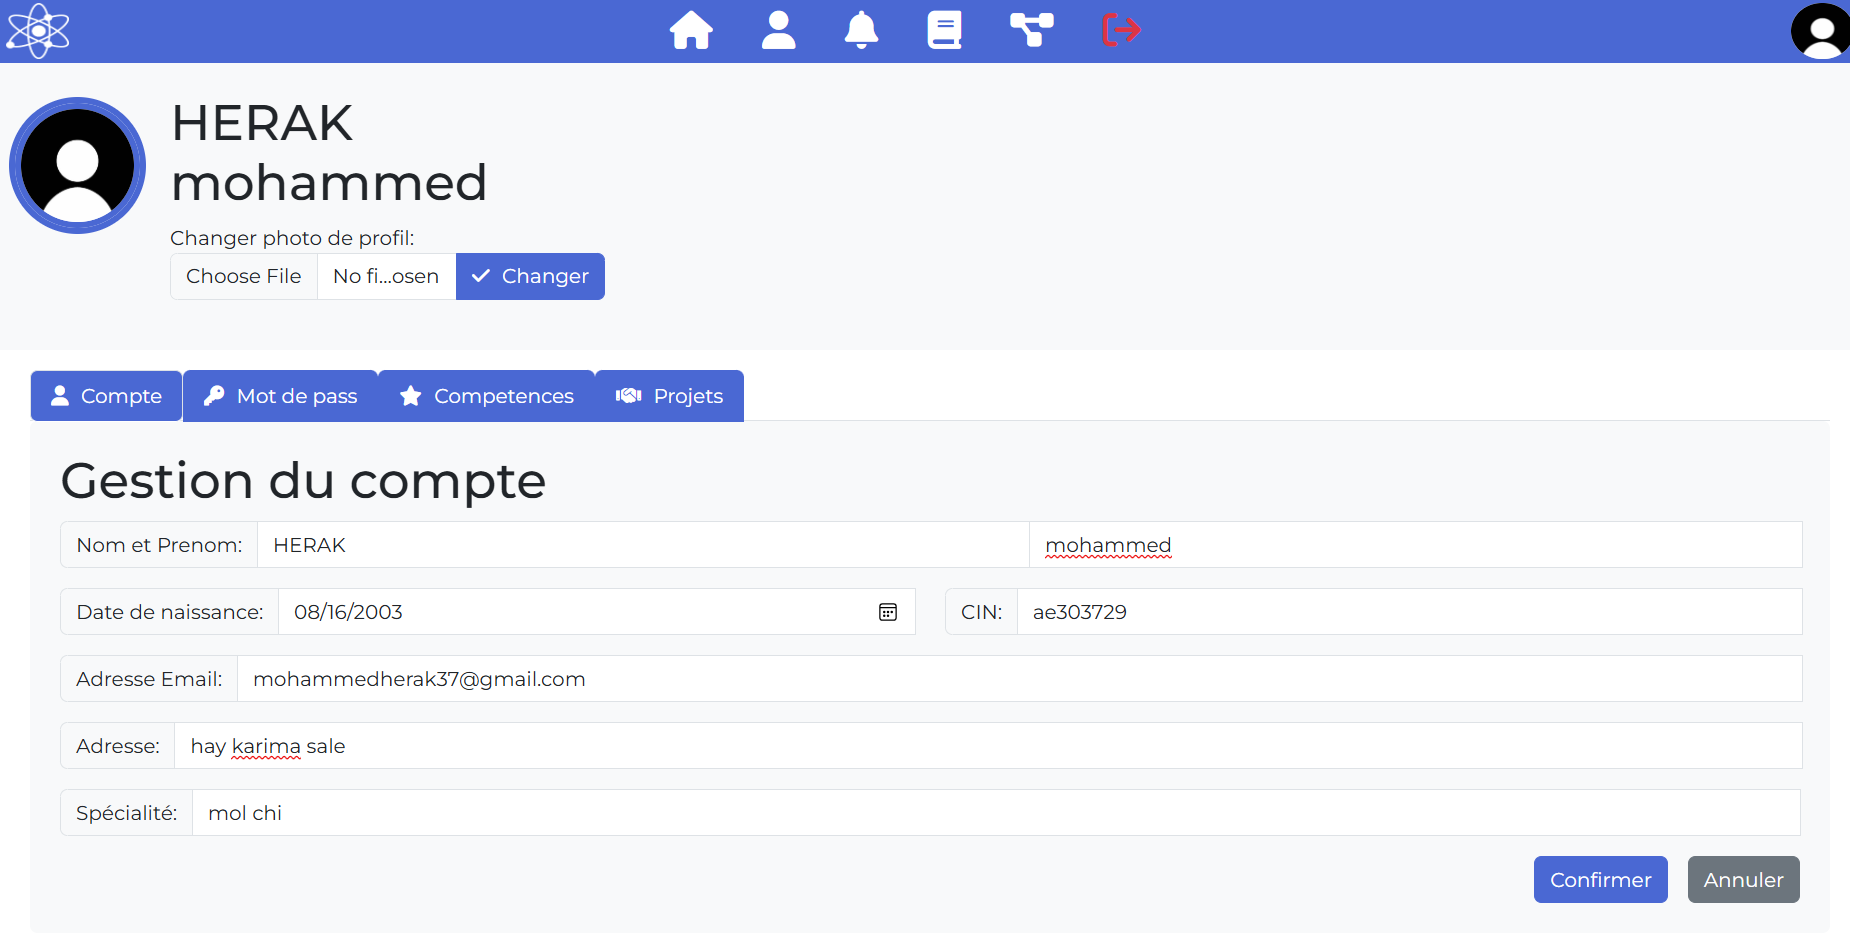
\includegraphics[width=0.8\textwidth]{assets/webSite/modifProfile.png}
                    \caption{Page de modification du profil}
                \end{figure}
                \FloatBarrier
            \subsubsection{Page des questions,formations et evenements}
                Cette page contient les questions poser par tous les collaborateurs, ainsi que les informations des formations et evenements disponibles, dans cette page le collaborateur peut ajouter et répondre a une question,ajouter ou/et s'interesser à une formation ou un evenement.
                \begin{figure}[h!]
                    \centering
                    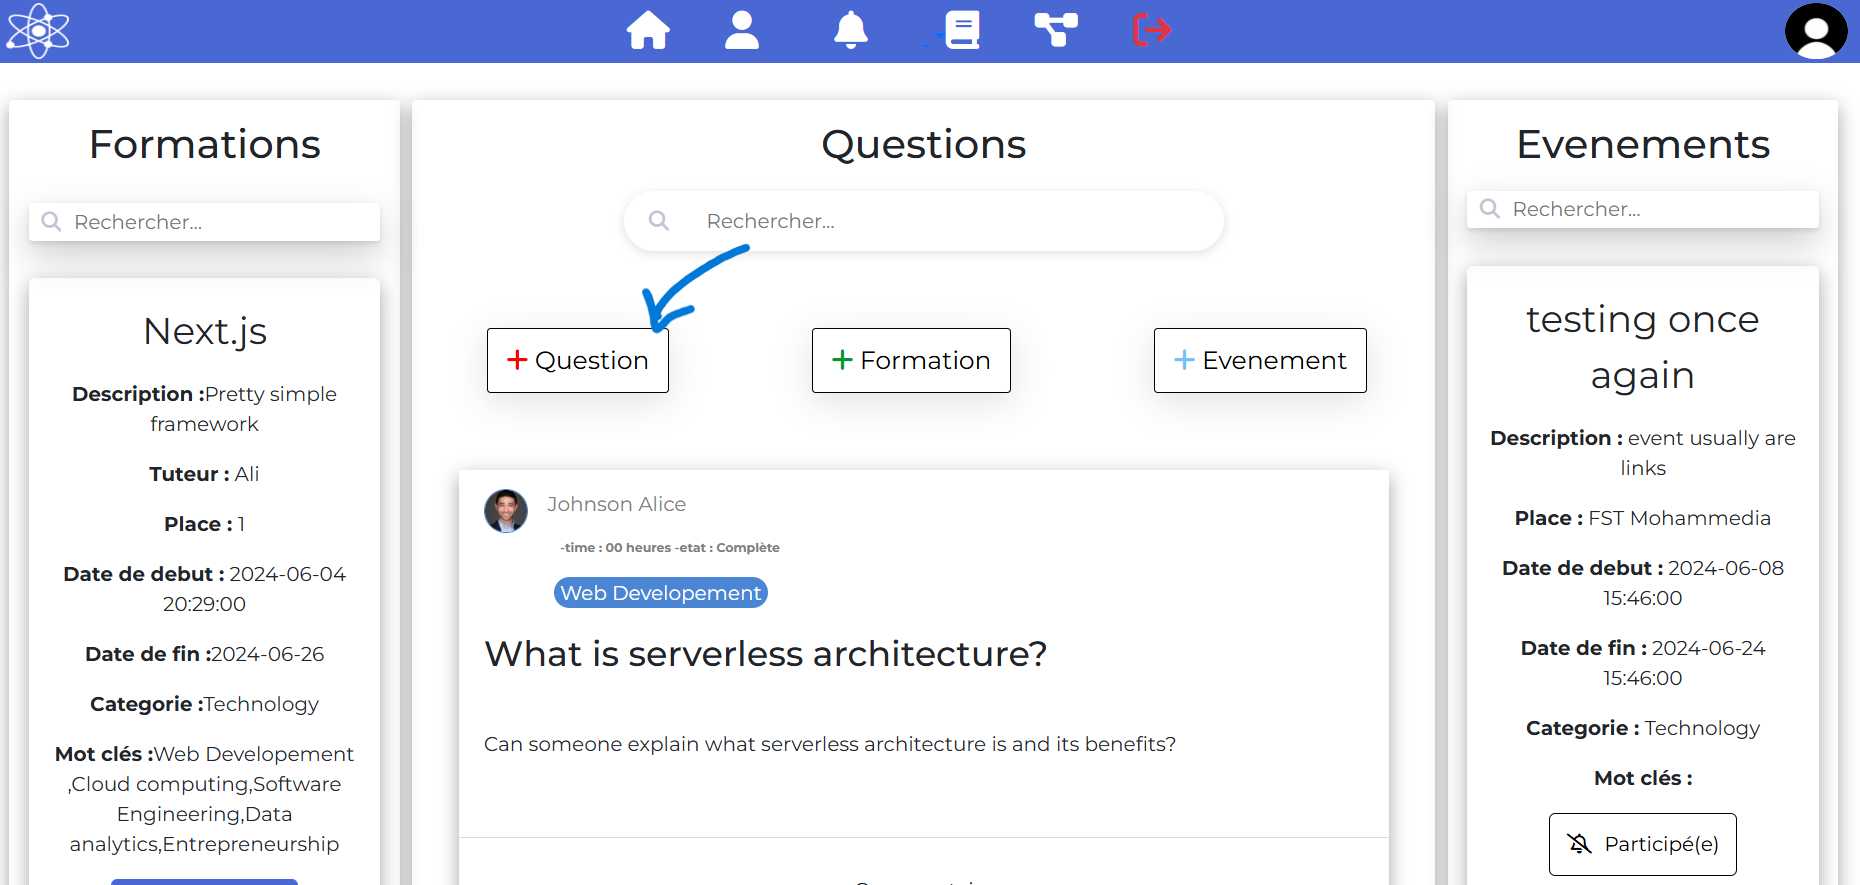
\includegraphics[width=0.8\textwidth]{assets/webSite/Acceuil.png}
                    \caption{Page des questions,formations et evenements}
                \end{figure}
                \FloatBarrier
                l'ajout d'une question ou bien un formation,evenement,projet et meme une connaissance se fait de la meme maniere, en cliquant sur le bouton correspondant en remplissant les informations, le formulaire est envoyer au serveur et traiter.
                \begin{figure}[h!]
                    \centering
                    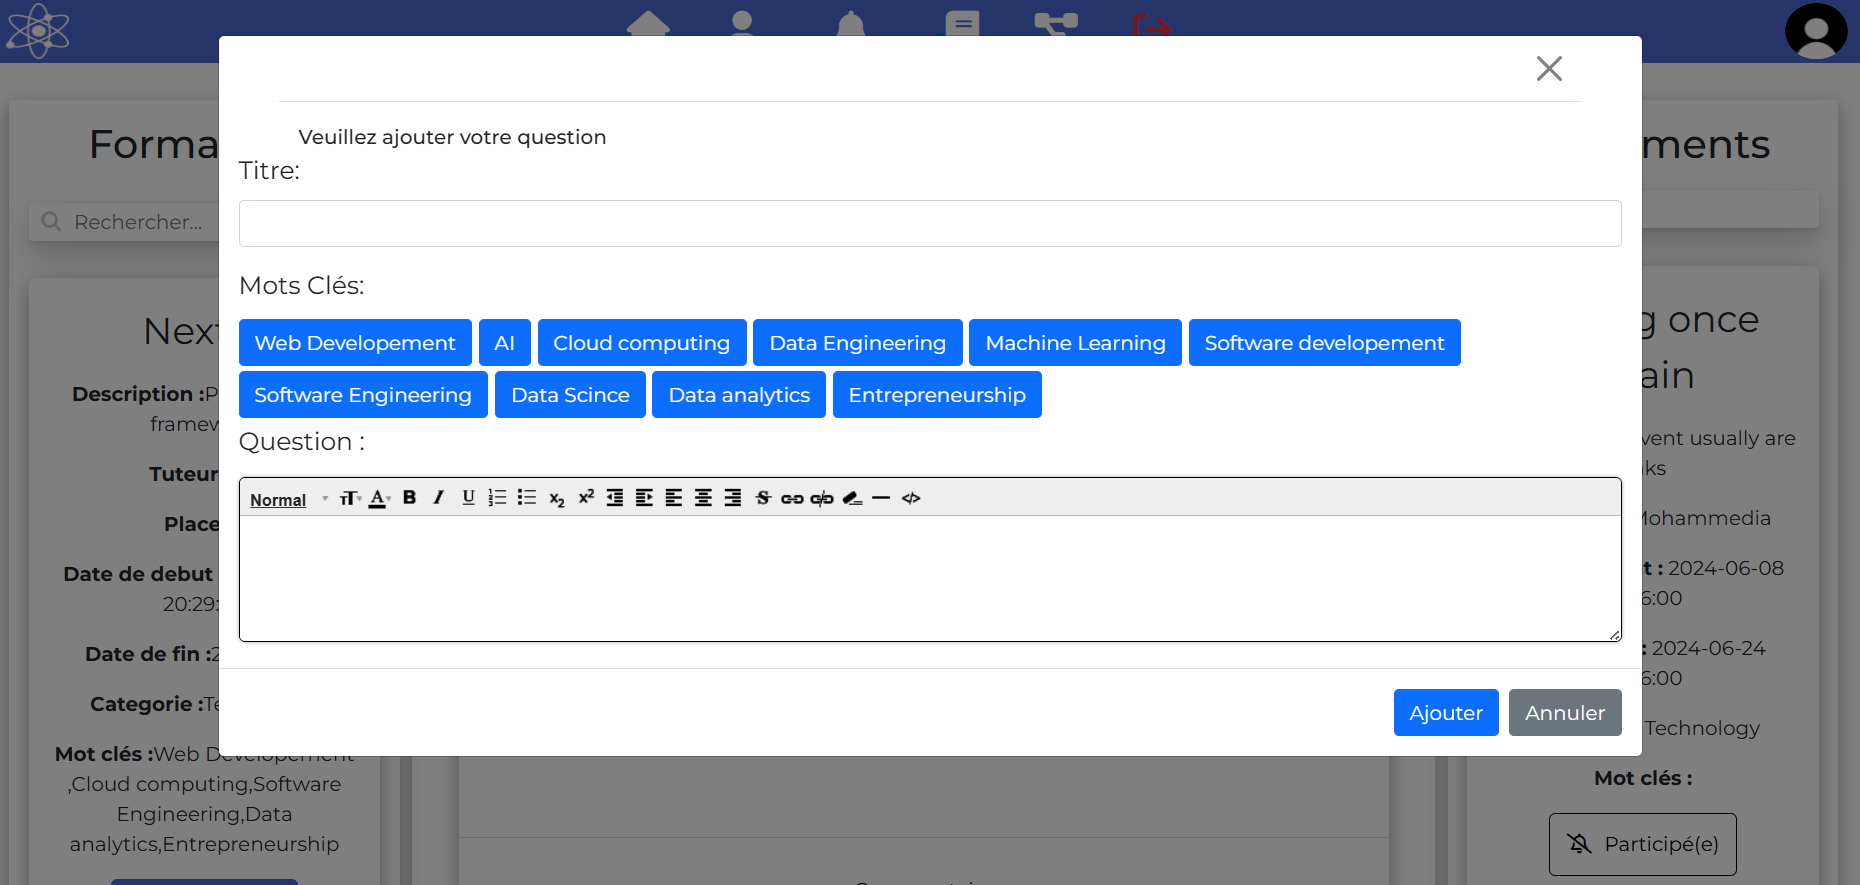
\includegraphics[width=0.8\textwidth]{assets/webSite/addQuestion.png}
                    \caption{Ajouter une question}
                \end{figure}
                \FloatBarrier
                Meme chose pour la recherche, le collaborateur peut effectuer une recherche par titre poue les questions,formations,evenements et connaissances.
                \begin{figure}[h!]
                    \centering
                    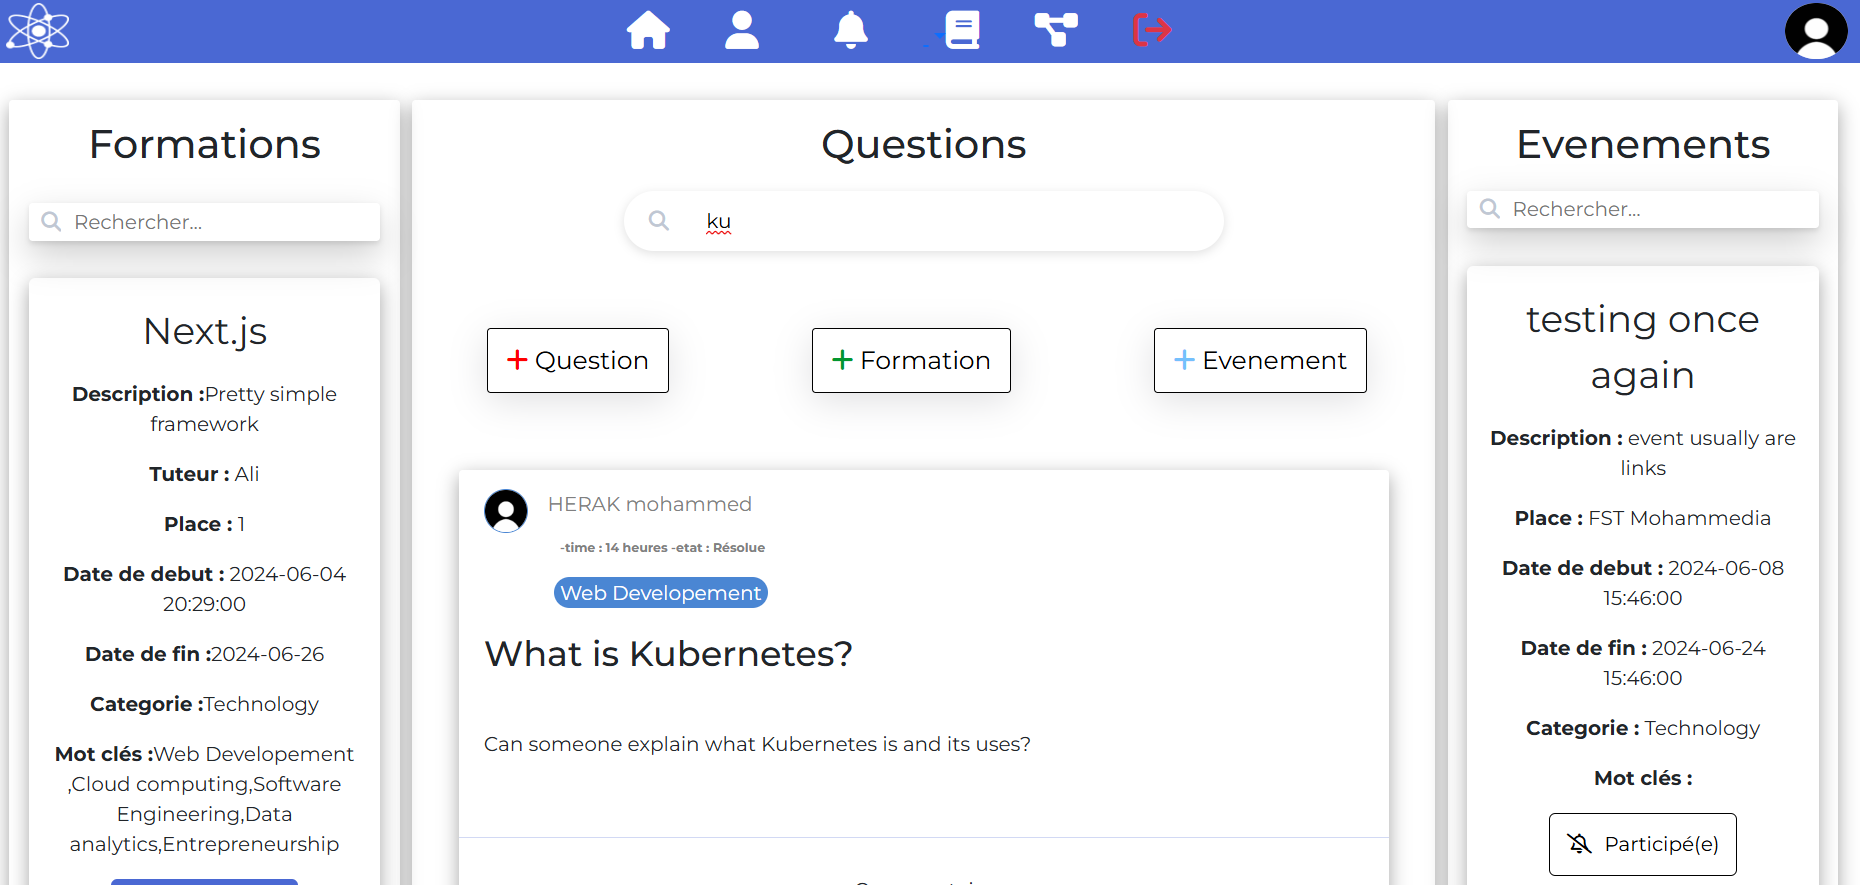
\includegraphics[width=0.8\textwidth]{assets/webSite/search.png}
                    \caption{Recherche}
                \end{figure}
                \FloatBarrier 
            \subsubsection{Page des connaissances}
                Le collaborateur peut acceder aussi a cet espace dedie aux connaissances, qui sont partager soit par lui meme soit par un autre collaborateur, aussi que ajouter des connaissances et les partager avec d'autres collaborateurs, la barre a gauche a pour but de simplifie la navigation.
                \begin{figure}[h!]
                    \centering
                    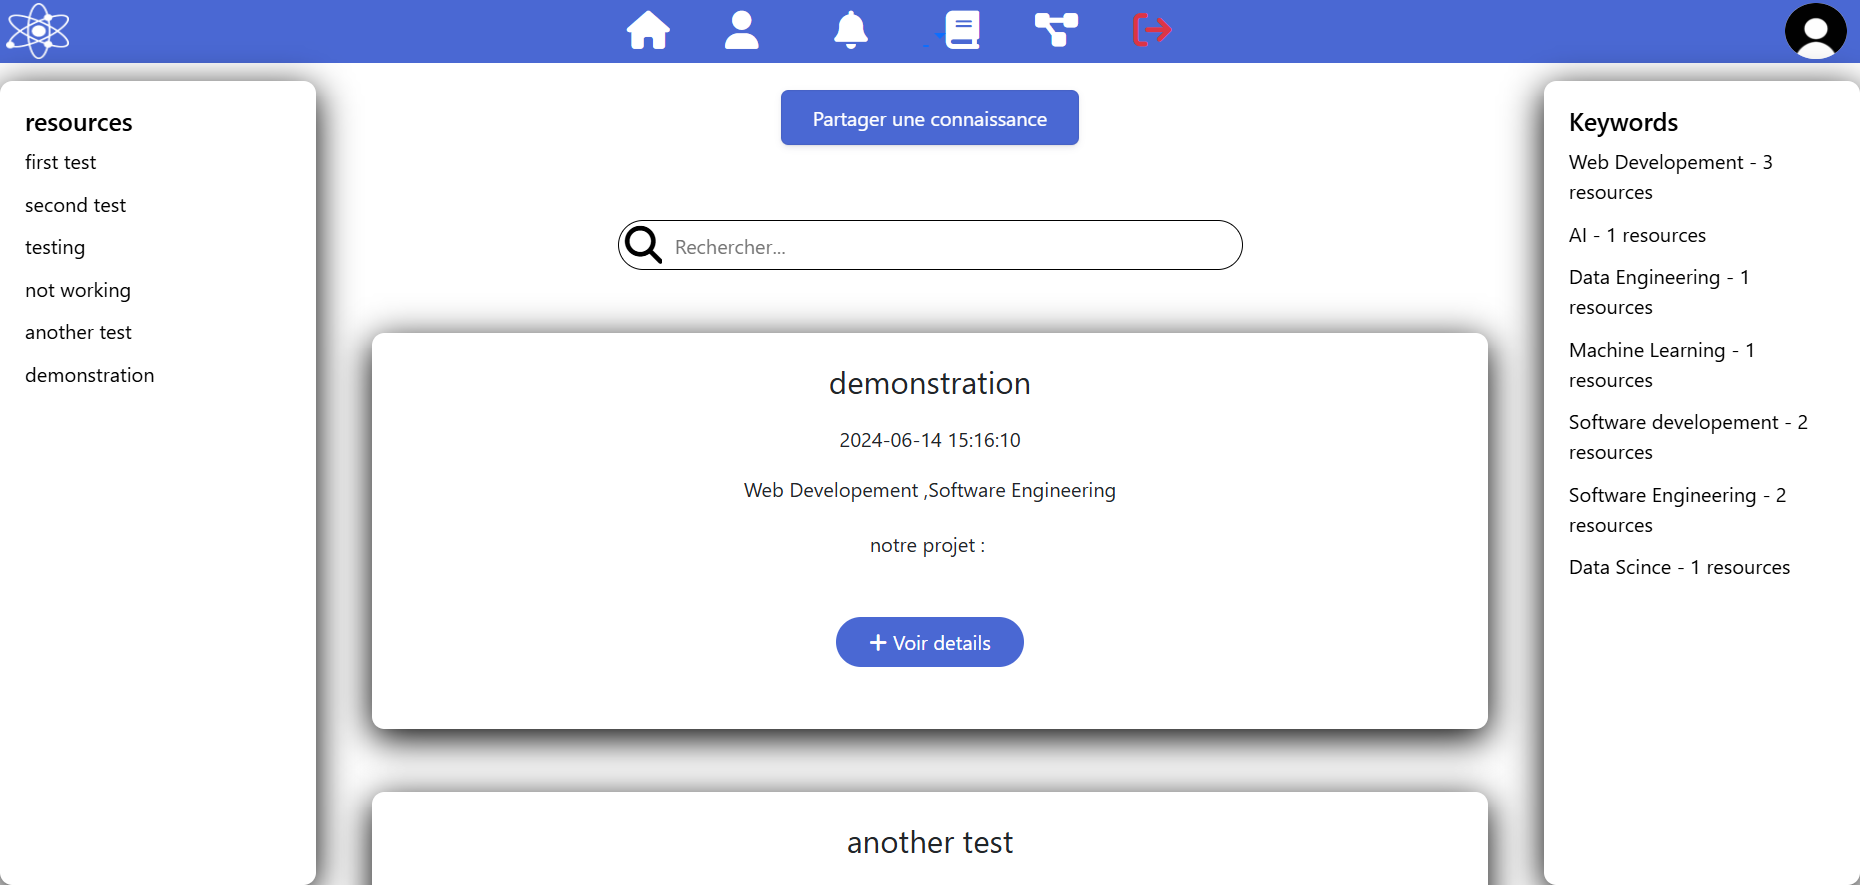
\includegraphics[width=0.8\textwidth]{assets/webSite/base-de-connaissance.png}
                    \caption{Page des connaissances}
                \end{figure}
                \FloatBarrier
                Pour ne pas charger la page des connaissances a chaque fois un utilisateur accéde sur la page, aucune connaissances n'est affichée sauf si le collaboteur clique sur  le bouton `voir details`,on affiche seulement les informations qui aide a identifie la connaissance  dans le debut.
                \begin{figure}[h!]
                    \centering
                    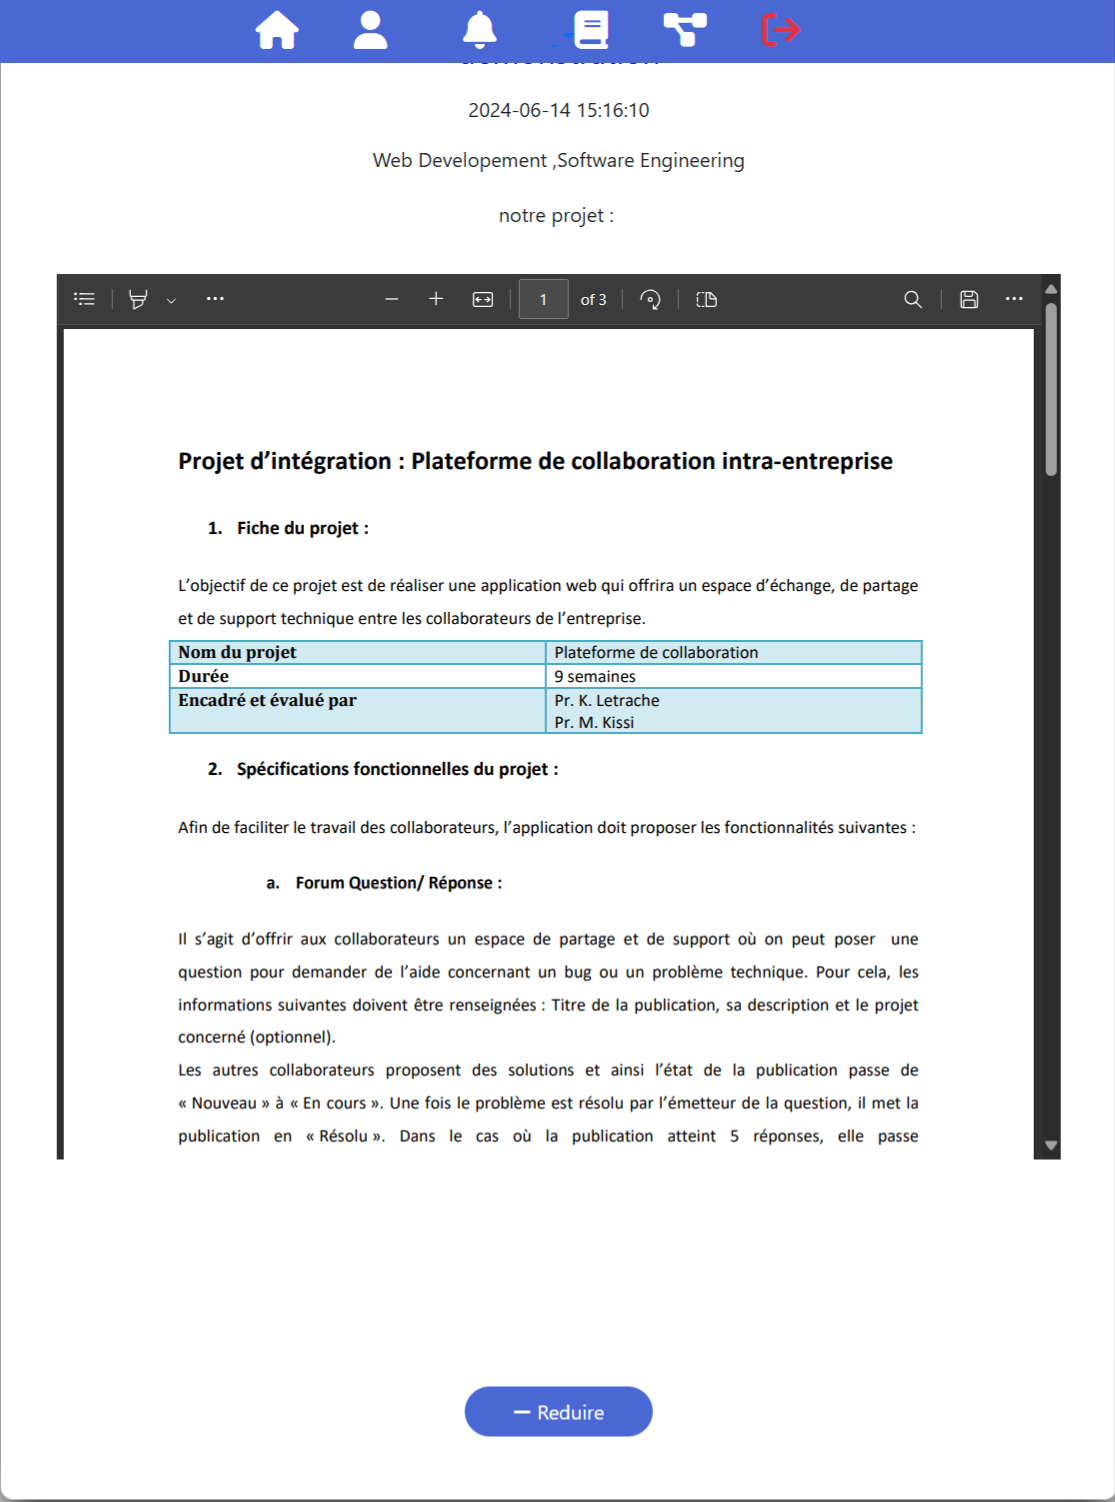
\includegraphics[width=0.8\textwidth]{assets/webSite/base-de-connaissance_demo.png}
                    \caption{des connaissances}
                \end{figure}
                \FloatBarrier
            \subsubsection{Page des projets}
                Là on a la page des projet, ou le collaborateur peut consulter les projets en cours.
                \begin{figure}[h!]
                    \centering
                    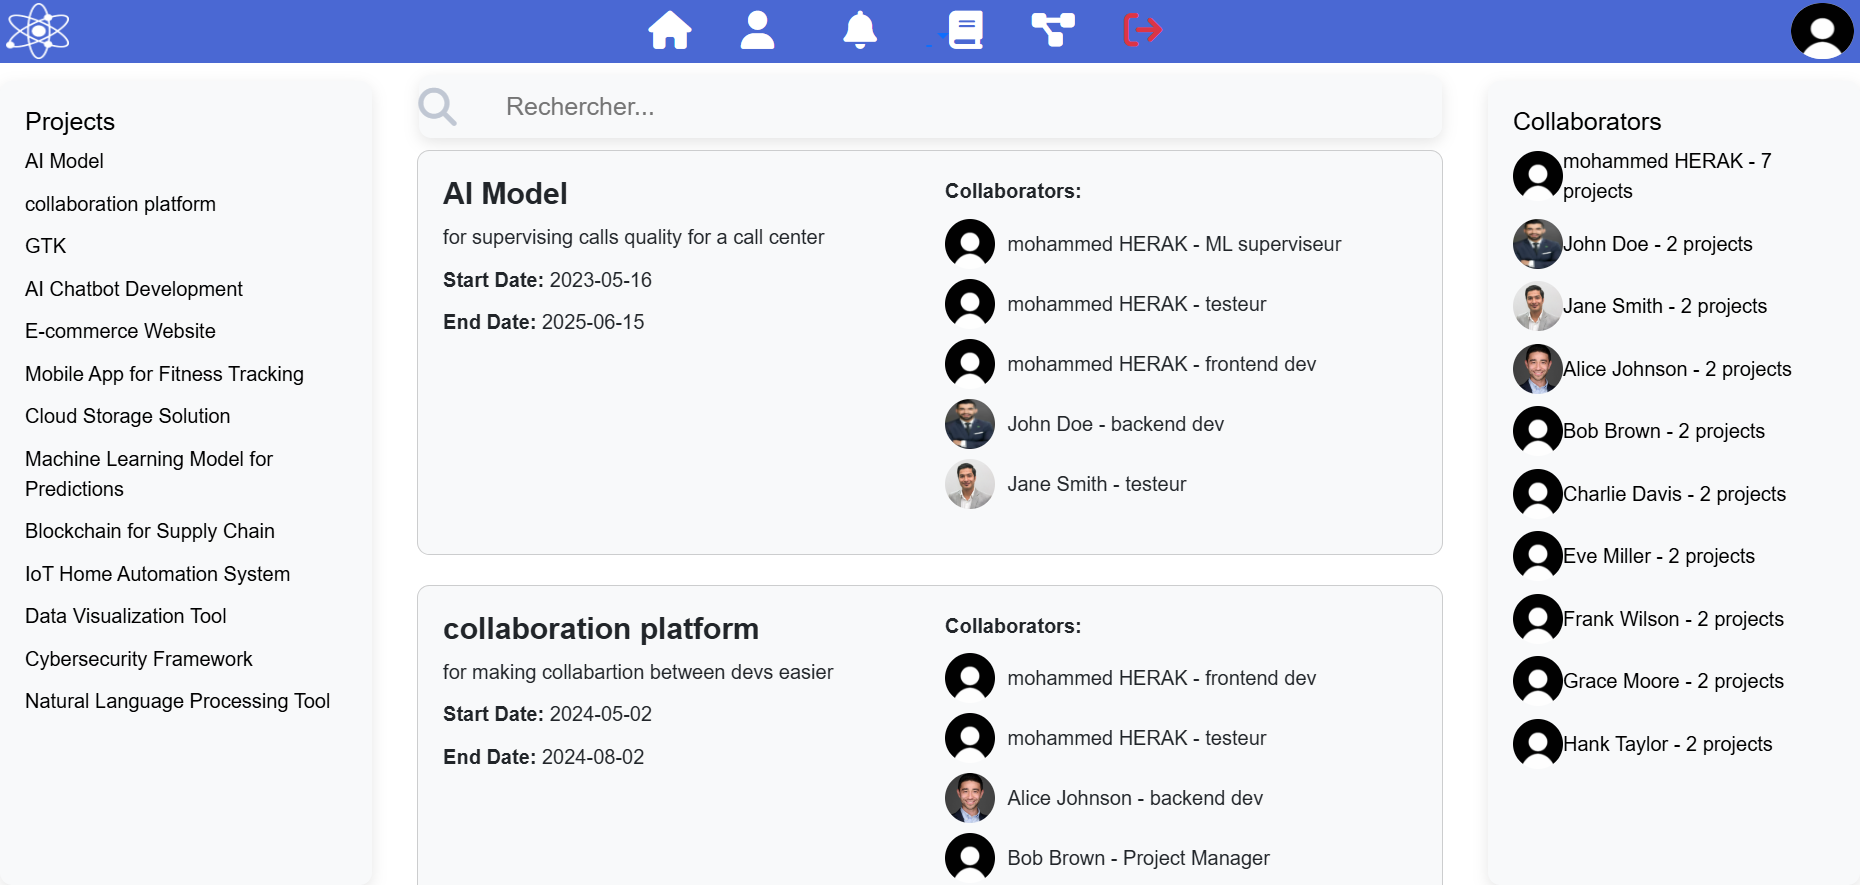
\includegraphics[width=0.8\textwidth]{assets/webSite/projectsPage.png}
                    \caption{Page des projets}
                \end{figure}
                \FloatBarrier
        \subsection{Espace Admin}
            \subsubsection{Page d'accueil}
            \subsubsection{Espace d'administration}
            \subsubsection{Page de modification du profil}
            \subsubsection{Dashboard}
    \section{Conclusion}
        
\end{document}